% -----------------------------------------------------------------------------
% Template from
% https://it.overleaf.com/articles/the-parallelization-and-optimization-of-the-n-body-problem-using-openmp-and-cuda/jpkcgbptkvby
% -----------------------------------------------------------------------------
\documentclass[letterpaper, 10 pt, conference]{ieeeconf}
\IEEEoverridecommandlockouts                              % This command is only
% needed if you want to
% use the \thanks command
\overrideIEEEmargins
% See the \addtolength command later in the file to balance the column lengths
% on the last page of the document


% The following packages can be found on http:\\www.ctan.org
\usepackage{graphics} % for pdf, bitmapped graphics files
\usepackage{epsfig} % for postscript graphics files
%\usepackage{mathptmx} % assumes new font selection scheme installed
%\usepackage{times} % assumes new font selection scheme installed
\usepackage{amsmath} % assumes amsmath package installed
\usepackage{amssymb}  % assumes amsmath package installed
\usepackage{booktabs}
\usepackage{caption}
\usepackage{url}
%\usepackage{algorithm}
\usepackage{verbatim}
%\usepackage[noend]{algpseudocode}
\usepackage{soul, color}
\usepackage{lmodern}
\usepackage{fancyhdr}
\usepackage[utf8]{inputenc}
\usepackage{fourier}
\usepackage{array}
\usepackage{makecell}

\renewcommand\theadalign{bc}
\renewcommand\theadfont{\bfseries}
\renewcommand\theadgape{\Gape[4pt]}
\renewcommand\cellgape{\Gape[4pt]}

\newcommand{\rework}[1]{\todo[color=yellow,inline]{#1}}

\makeatletter
\newcommand{\rom}[1]{\romannumeral #1}
\newcommand{\Rom}[1]{\expandafter\@slowromancap\romannumeral #1@}
\makeatother

\pagestyle{plain}

\title{\LARGE \bf
Analysis of the Spatial Covariance Shift in Weather Inference
}
\author{Simone PAPICCHIO, Federico TIBLIAS, Massimo PRONESTI, Daniele FALCETTA% <-this % stops a space 
\\EURECOM - Department of Data Science \\
Sophia Antipolis, France\\
{\tt\small\{name.surname\}@eurecom.fr} \\ \\
}


\begin{document}


    \maketitle
    \thispagestyle{plain}
    \pagestyle{plain}


%%%%%%%%%%%%%%%%%%%%%%%%%%%%%%%%%%%%%%%%%%%%%%%%%%%%%%%%%%%%%%%%%%%%%%%%%%%%%%%%
\begin{abstract}
   The Weather Forecast problem consists in using climatic measurements and predictions from different models in order to predict the air temperature measurement at 2 metres above the ground. The dataset shows highly correlated features and a serious shift between train and test distributions. Our approach to address these issues start with the analysis of the dataset and, in particular, outliers, correlation and feature shift. Subsequently, we run differents experiments using several distinct preprocessing techniques such as scaling, feature selection and PCA. In the end we select the best model through a grid search and settle for a solution based on XXX and YYY that outperforms all other examined models.
\end{abstract}

\section{INTRODUCTION}
    The Weather Forecast problem consists in using climatic measurements and predictions from different models (Global Forecast System, Global Deterministic Forecast System from the Canadian Meteorological Center, Weather Research and Forecasting) in order to predict the air temperature measurement at 2 metres above the ground. The dataset shows highly correlated features and a serious shift between train and test distributions.
    When the distribution of the train and test data differs, this is known as dataset shifting. This may cause several problems because the model is trained on one distribution but is used to make predictions on a different one, resulting in poor results. There are different types of data shifting such as 
    Covariance Shift\footnote{Changes in the independent variables or features of the dataset},
    Probability Shift\footnote{Changes in the target variable or the dependent variable in the dataset}
    and Concept Shift.\footnote{Change in the connection between the independent and the target variable across datasets}
    In this work we analyze the presence of the Spatial Covariance Shift and try to address its main challenges.

    The data consists of pairs of meteorological features and target values at a particular latitude/longitude and time. The Regression task consists in predicting the air temperature measurements at 2 meters above the ground.
    The features are either direct measurements (such as sun elevation at the current location, humidity, temperature, pressure and topography, and other meteorological parameters) or weather predictions provided by climatic models (Global Forecast System, Global Deterministic Forecast System from the Canadian Meteorological Center, Weather Research and Forecasting)
    Each model returns the following predicted values: wind, humidity, pressure, clouds, precipitation, dew point, snow depth, air and soil temperature characteristics. Where applicable, the predictions are given at different isobaric levels from 50 hPa (20 km above ground) to the ground level.

    Altogether, there are 111 features in total. It is important to note that the features are highly heterogeneous, i.e., they are of different types and scales.

    The main challenge of this dataset is the Spatial Covariance Shift from train to test as visible in Fig. \ref{fig:train-test-diff}

    \begin{figure}
        \centering
        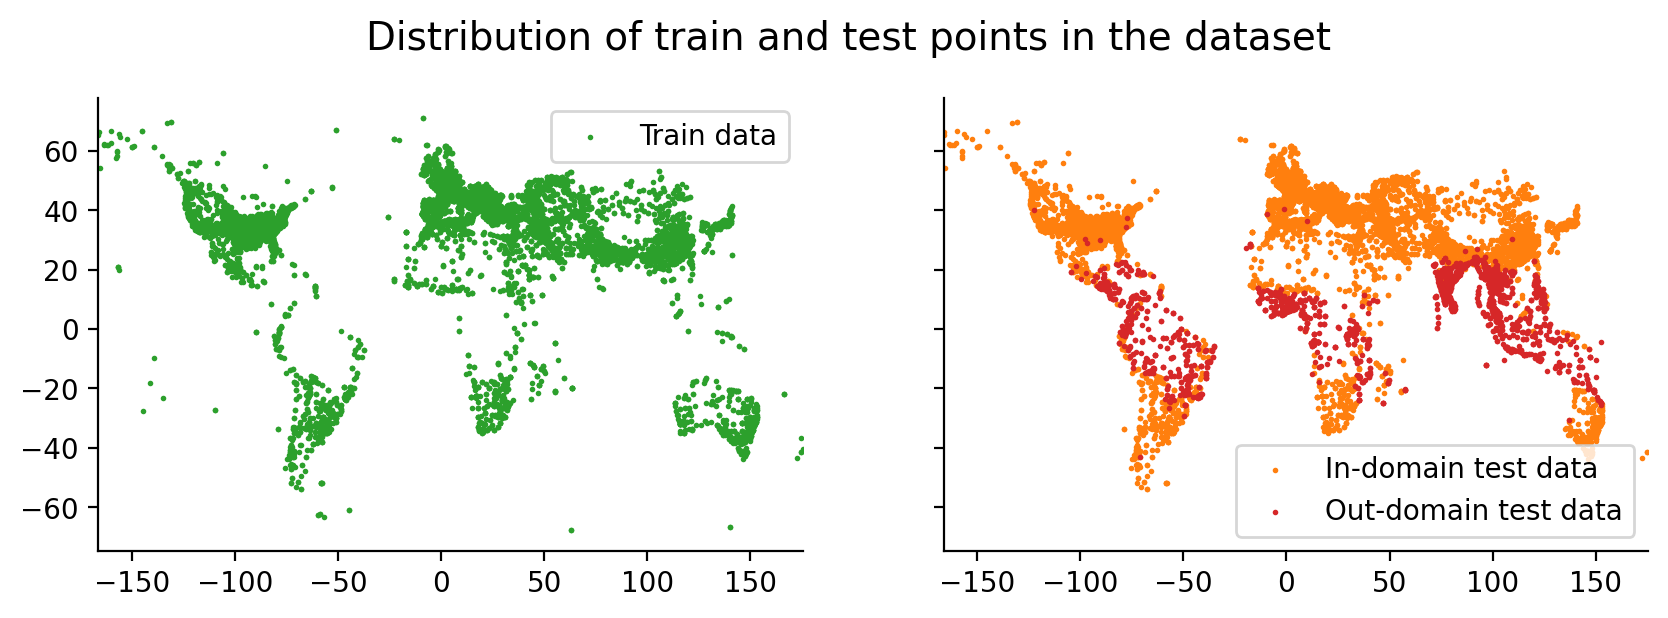
\includegraphics[width=\linewidth]{assets/train-test-diff.png}
        \caption{The figure clearly shows that the regions in the range of latitude from -18 to 10 are not present in the train dataset. This phenomenon is called \textit{Spatial Covariance Shift}. [best visualization in colors] }
        \label{fig:train-test-diff}
    \end{figure}

    \section{Data Analysis}
    
    \subsection{Outliers}
    The first step of our dataset analysis focuses on the outliers detection. Our approach, based on the Interquartile method (IQR), consists in plotting a boxplot for each feature. To obtain better and more organized visualization we decided to plot four different graphs, one for each weather forecast model and, given the high heterogeneity of the features, we decided to scale our data between 0 and 1 according to a min-max normalization.
    From the analysis of the plots we can notice that almost all the features contain some outliers. Below, in the models section, we run some experiments in which we tried to remove part or all of them. A particular mention has to be done for the feature \textit{gfs\_soil\_temperature} which min value is \textit{-9999 C}, an impossible value for a temperature in the whole universe.
    \subsection{Correlations}
    Important for the analysis is to understand the correlations present in the dataset. We start analyzing the correlation between the features and the target. 
    
\setlength{\tabcolsep}{3em}
\begin{table}
\begin{center}
\begin{tabular}{lccl}
\toprule
Feature                         & Pearson Correlation \\ \midrule
\textbf{wrf\_t2\_interpolated}   & \textbf{0.963}     \\
wrf\_t2\_next                   & 0.958               \\
gfs\_temperature\_97500         & 0.874               \\
gfs\_temperature\_95000         & 0.863               \\
climate\_temperature            & 0.857               \\
gfs\_temperature\_92500         & 0.852               \\
gfs\_temperature\_90000         & 0.842               \\
gfs\_temperature\_85000         & 0.824               \\
gfs\_temperature\_80000         & 0.808               \\
cmc\_0\_0\_6\_2                 & 0.807               \\ \bottomrule
\end{tabular}
\end{center}
\captionof{table}{Most correlated feature according to the Pearson metric. AAAAAAAAAAAAAAA} 
\end{table}
    
    
    \subsection{Feature Shift}
    Train and test datasets show a noticeable shift in the distribution of samples: test datapoints are distributed homogeneously around the globe, while train ones are only 
    To gain a deeper understanding of how this phenomenon affects our prediction we compute a metric reminiscent of the Wasserstein distance. For each feature we divide the dataset into 100 bins of equal size and normalize them in order to obtain histograms. Then, we compute the area difference between the cumulative sum of these histograms for train and test datasets. The value we obtain represents some notion of distance between the two distributions and can be used later on during feature selection. We report in Table I the 10 most shifted features according to this metric. 
\setlength{\tabcolsep}{2em}
\begin{table}
\begin{center}
\begin{tabular}{lccl}
\toprule
Feature                         & Wasserstein distance \\ \midrule
fact\_latitude                  & 13.625               \\
gfs\_total\_clouds\_cover\_high & 13.718               \\
gfs\_temperature\_15000         & 14.541               \\
gfs\_v\_wind                    & 16.866               \\
gfs\_precipitable\_water        & 16.999               \\
cmc\_0\_1\_0\_0                 & 17.057               \\
gfs\_2m\_dewpoint\_grad         & 24.006               \\
cmc\_available                  & 49.000               \\
gfs\_available                  & 49.000               \\
wrf\_available                  & 49.000               \\ \bottomrule
\end{tabular}
\end{center}
\captionof{table}{Most shifted features between train and test dataset according to Wasserstein metric.} 
\end{table}

    \section{Pre-Processing}
    Different models call for different preprocessings and feature selections. We try different approaches in conjunction with one or more models to find the best one in each situation.
    \begin{itemize}
        \item \textbf{Dealing with missing values:} either fill missing values with their respective column mean or drop samples containing at least one NaN.
        \item \textbf{Outlier removal} either using the interquartile method or on the local outlier factor.
        \item \textbf{Rescaling:} normalize all features using sklearn's \textit{StandardScaler}.
        \item \textbf{Feature selection based on Random Forest feature importance:} train a Random Forest to predict the target value and  keep only the $n$ most important features according to the model. Use these selected features with another model.
        % Fill in the others.
        \item \textbf{Feature selection based on Wasserstein distance:} rank features according to the metric described in the previous section and keep only the $n$ less shifted ones as they should better represent the test distribution.
        \item \textbf{PCA:} correlation analysis shows many features are correlated, this poses a problem for linear models. We address this issue by performing a PCA keeping either \textit{num\_features} - 1 principal components or by selecting the components explaining $99\%$ of variance.
        \item \textbf{Daylight and hour:} use \textit{fact\_time, fact\_latitude, fact\_longitude} to compute amount of daylight received and hour the measurement took place.
    \end{itemize} 
    
    \section{Models}
    We perform an initial exploratory analysis comparing a variety of models along with different preprocessings and pick the ones that perform best to be further explored with hyper-parameter tuning. 
    
    
    
    The models we compared are:
    \begin{itemize}
        \item \textbf{Ridge:} Gives promising results but is susceptible to collinearity. PCA is always required to train it. Removing most shifted features seems to positively affect performances.
        \item \textbf{Random Forest:} Robust to outliers and gives good performance for a small number of estimators. The downside is its training time.
        \item \textbf{Catboost:} Performs very well without any feature selection or PCA required. Being an ensemble method it's much more difficult to interpret, training takes a long time.
        \item \textbf{Gradient boosting regressor:} Same issues as Catboost but we observe worst performances.
        \item \textbf{Support vector regressor:} Training takes an unfeasible amount of time.
    \end{itemize} 
    
    
    
    \section{Hyper-parameter tuning}
    After our initial exploratory model analysis we fix the preprocessing that better performs in combination to a certain model and perform tuning over the model's hyper-parameters. To do this we rely on sklearn's XXXCV %Fill in missing name
    
    A list of hyper-parameters we compared for each model can be found in Table X.
    
\begin{table*}[t]
\begin{center}
\begin{tabular}{lp{2cm}p{2cm}p{3cm}ccl}
\toprule
%THESE ARE ONLY PLACEHOLDER VALUES, FILL IN CORRECT ONES
Preprocessing \& Model    & Hyperparameters explored & Best hyperparameters & Validation score & Test score (Kaggle)\\ \midrule
StandardScaler, PCA, Ridge & alpha: [0.1, 0.01, 0.001] & alpha: 0.1 & 0.420 & 0.690\\
StandardScaler, Random Forest & \makecell{num\_iterations: [10, 25, 20] \\ max\_depth: [3, 6, 9]} & \makecell{num\_iterations: 10 \\ max\_depth: 3} & 0.420 & 0.690\\ \bottomrule
\end{tabular}
\end{center}
\captionof{table}{Models and hyperparameters tested.} 
\end{table*}
    
    
    \section{Results}
    By applying different combinations of preprocessing we observed the following:
    \begin{itemize} 
        \item Filling missing values with the column mean or dropping the sample altogether produced comparable results. We chose to always fill with the mean to avoid dropping potentially useful samples
        \item Although we tried different outliers removal techniques over distinct experiments, we obtained our best results by keeping the outliers in the analysis.
        \item Rescaling proves always useful in improving performances.
        \item Despite our efforts in coming up with sensible metrics for feature selection we find that keeping all features and letting the model choose the most important ones during training is still the best-performing approach. 
        \item PCA is needed only for linear models to avoid collinearity. Other models show a reduction in performance when PCA is applied.
        \item Daylight and hour don't lead to any noticeable improvements on any analyzed model. 
    \end{itemize} 

    
    
    \section{Conclusions}
    %Future works
    Despite consisting of almost 2 million measurements, the actual weather stations are few in number, totaling around 5000. A more detailed analysis could investigate aggregates of measurements coming from the same station in order to increase performance. An even more refined approach would be to group together measurements coming from the same station and treat the prediction as a time series problem, applying models such as RNNs and LSTM.
    
%%%%%%%%%%%%%%%%%%%%%%%%%%%%%%%%%%%%%%%%%%%%%%%%%%%%%%%%%%%%%%%%%%%%%%%%%%%%%%%%

\end{document}
